% Déclaration du type de document (report, book, paper, etc...)
\documentclass[a4paper, 12pt]{paper} 
 
% Package pour avoir Latex en français
\usepackage[utf8]{inputenc}
\usepackage[T1]{fontenc}
 
% Quelques packages utiles
\usepackage{listings} % Pour afficher des listings de programmes
\usepackage{graphicx} % Pour afficher des figures
\usepackage{amsthm}   % Pour créer des théorèmes et des définitions
\usepackage{amsmath}
\usepackage{microtype} % Optical margins FTW
\usepackage{url}
\usepackage{booktabs} % Allows the use of \toprule, \midrule and \bottomrule in tables for horizontal lines
\usepackage[per-mode=symbol]{siunitx}
\usepackage{floatrow}
\usepackage{caption}
\usepackage{subcaption}
\usepackage{fullpage}
\usepackage{lipsum}



\author{Loïc Amez-Droz \and Florian Reinhard}
\title{Imaging}

% Début du document
\begin{document}
\begin{titlepage}
\begin{center}
    \textsc{\LARGE École Polytechnique Fédérale de~Lausanne}\\[1.5cm] 
    {\huge \bfseries Optical Engineering: Multimode Fibre}\\[0.4cm] 
    \begin{tabular}{|p{5cm}|p{4cm}|}
        \hline
        Group & C-XX \\ \hline
        Students & Loïc \textsc{Amez-Droz} \newline Florian \textsc{Reinhard} \\ \hline
        Date of lecture & 13.03.2015 \\ \hline
        Date of final report return & 20.03.2015 \\ \hline
    \end{tabular}
\end{center}


\begin{abstract}
    \lipsum[3]
\end{abstract}
 
\vfill
\end{titlepage}

\section{Minimal source focusing}
\subsection{Measurement with the Logitech C600 camera objective}
Placing sources away from the camera, we evaluate the smallest focus size that can be obtained by sources.
The distance between the source and the camera is $s_O = \SI{208}{\milli\meter}$.
These diameters in millimeters are converted knowing the properties of the sensor.
A pixel represents $c = \SI{2.835}{\micro\meter}$.
The magnification factor $m = \frac{r_I}{r_O} = \frac{4.536}{208} = \SI{21.8e-3}{}$

\begin{equation}
    \Delta m = \frac{r_I}{r_O^2} \Delta r_O = \frac{4.536}{208^2}2 = \SI{2.1e-4}{}
\label{equ:m_err}
\end{equation}

\begin{equation}
    \frac{\Delta m}{m} = \SI{1}{\percent}
\label{equ:m_err_percent}
\end{equation}

The error of the Matlab plot is estimated to be $\Delta d_I = 1\mbox{px}$.

\paragraph{Diameter of the source point}

\begin{equation}
    d_O = \frac{c}{m} d_I
    \label{equ:object_diam}
\end{equation}

\begin{equation}
    \Delta d_O = \frac{c}{m} \Delta d_I + \frac{d_I c}{m^2} \Delta m
    = \frac{d_O}{d_I} \Delta d_I + \frac{d_O}{m} \Delta m
    = d_O \left( \frac{1}{d_I} + \SI{9.6e-3}{} \right)
    \label{equ:object_diam_err}
\end{equation}

\begin{table}[h]
    \centering
    \begin{tabular}{l S[table-format=1.0] S[table-format=1.2] S[table-format=1.2] S[table-format=2.1]}
        \toprule
        source & {image space $d_I$ (px)} & {object space $d_O$ (\SI{}{\milli\meter})} & {$\Delta d_O$} & {error (\SI{}{\percent})} \\
        \midrule
        Halogen & 27 & 3.51 & 0.16 &  4.6 \\
        LED     & 25 & 3.25 & 0.16 &  4.9 \\
        Laser   &  6 & 0.78 & 0.14 & 17.9 \\
        \bottomrule
    \end{tabular}
    \caption{Diameter of the source point.}
\label{tab:diams}
\end{table}

\begin{figure}[h]
    \centering
    \begin{subfigure}[p]{0.30\textwidth}
        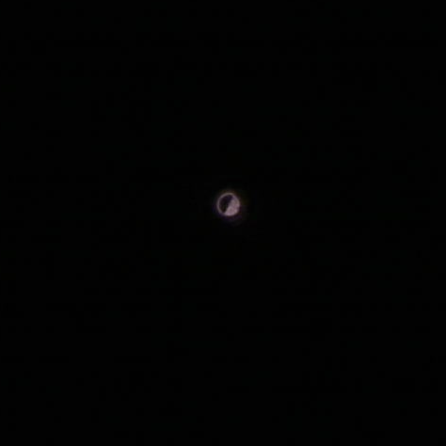
\includegraphics[width=\textwidth]{img/halogen_source}
        \caption{Halogen source.}
    \end{subfigure}
    \begin{subfigure}[p]{0.30\textwidth}
        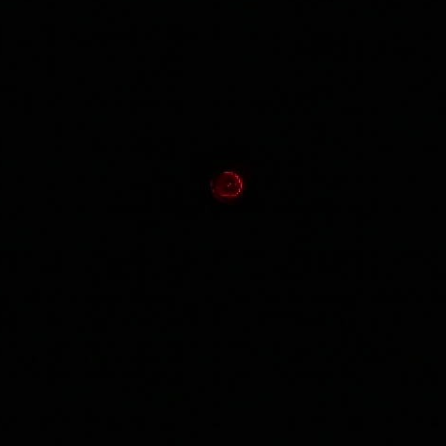
\includegraphics[width=\textwidth]{img/led_source}
        \caption{LED source.}
    \end{subfigure}
    \begin{subfigure}[p]{0.30\textwidth}
        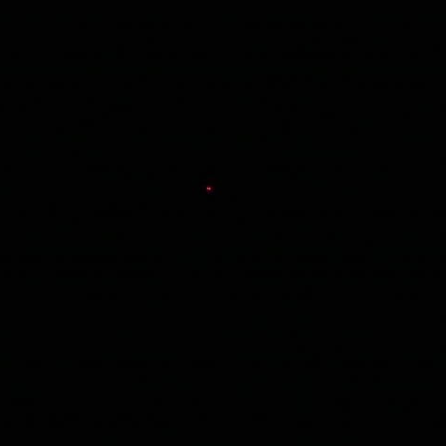
\includegraphics[width=\textwidth]{img/laser_source}
        \caption{Laser source.}
    \end{subfigure}
    \caption{Images taken to measure the diameter of the source point.}
\label{fig:source_points}
\end{figure}

\subsection{Evaluating focusing with a planconvex lens}

Substituting the objective lens by a planconvex lens, which has a greater focal length, we obtain a greater source picture on the sensor.
The halogen filament as well as the chip and its bonding wire are perceptible.

\begin{figure}[h]
    \centering
    \begin{subfigure}[p]{0.40\textwidth}
        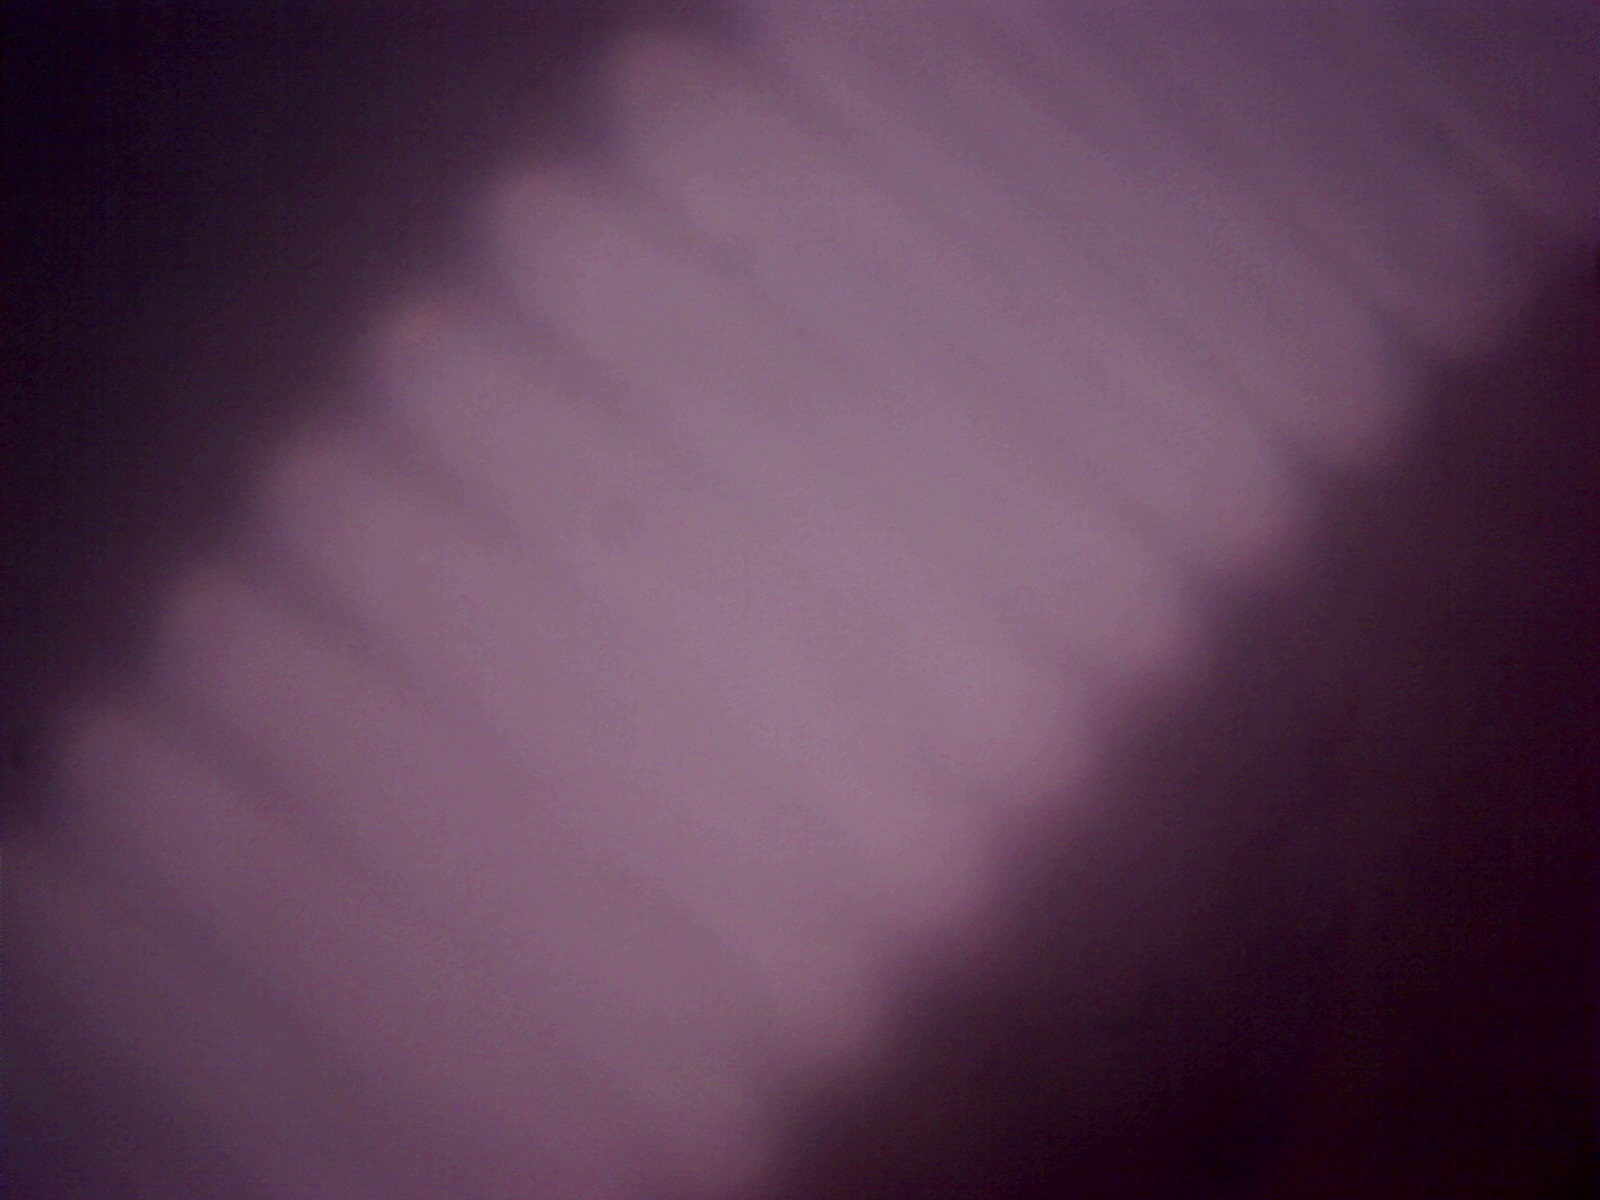
\includegraphics[width=\textwidth]{img/lens_halogen}
        \caption{Halogen filament.}
    \end{subfigure}
    \begin{subfigure}[p]{0.40\textwidth}
        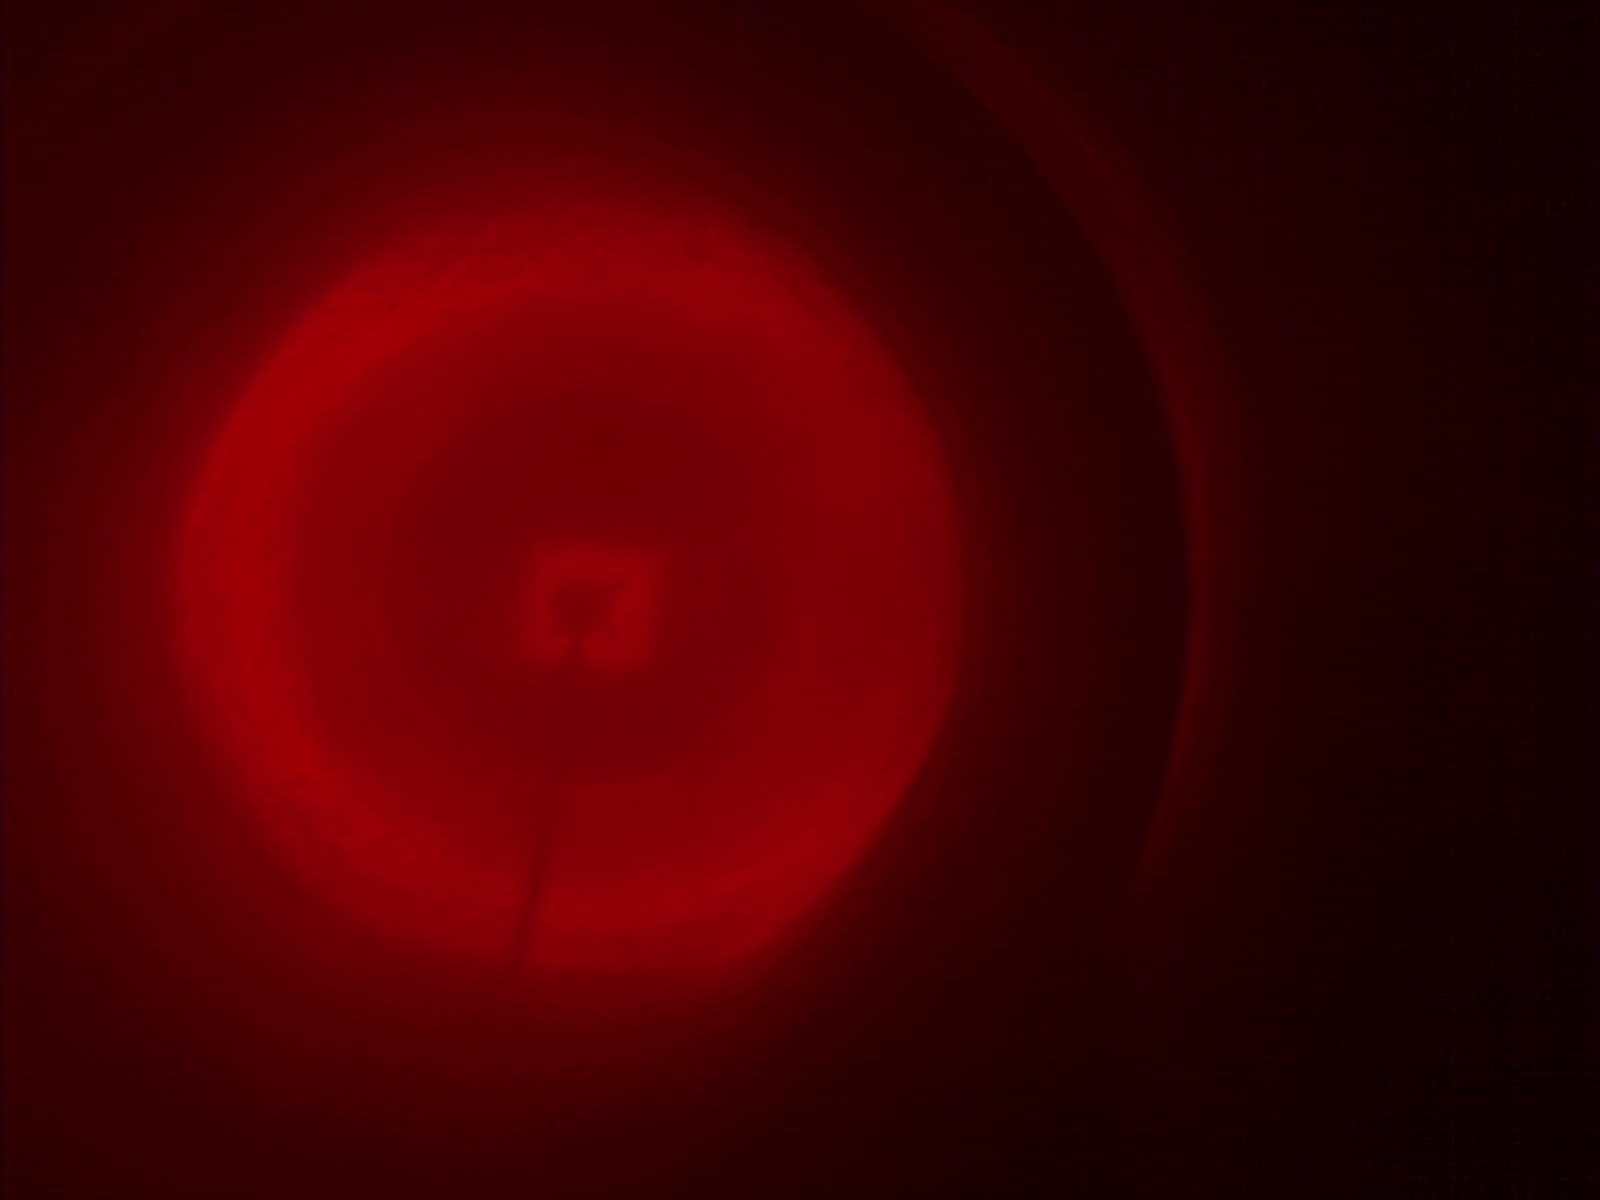
\includegraphics[width=\textwidth]{img/lens_led}
        \caption{LED chip.}
    \end{subfigure}
    \caption{Close up images of the sources through the planconvex lens.}
\label{fig:planconvex}
\end{figure}

\begin{figure}[h]
    \centering
    \begin{subfigure}[p]{0.30\textwidth}
        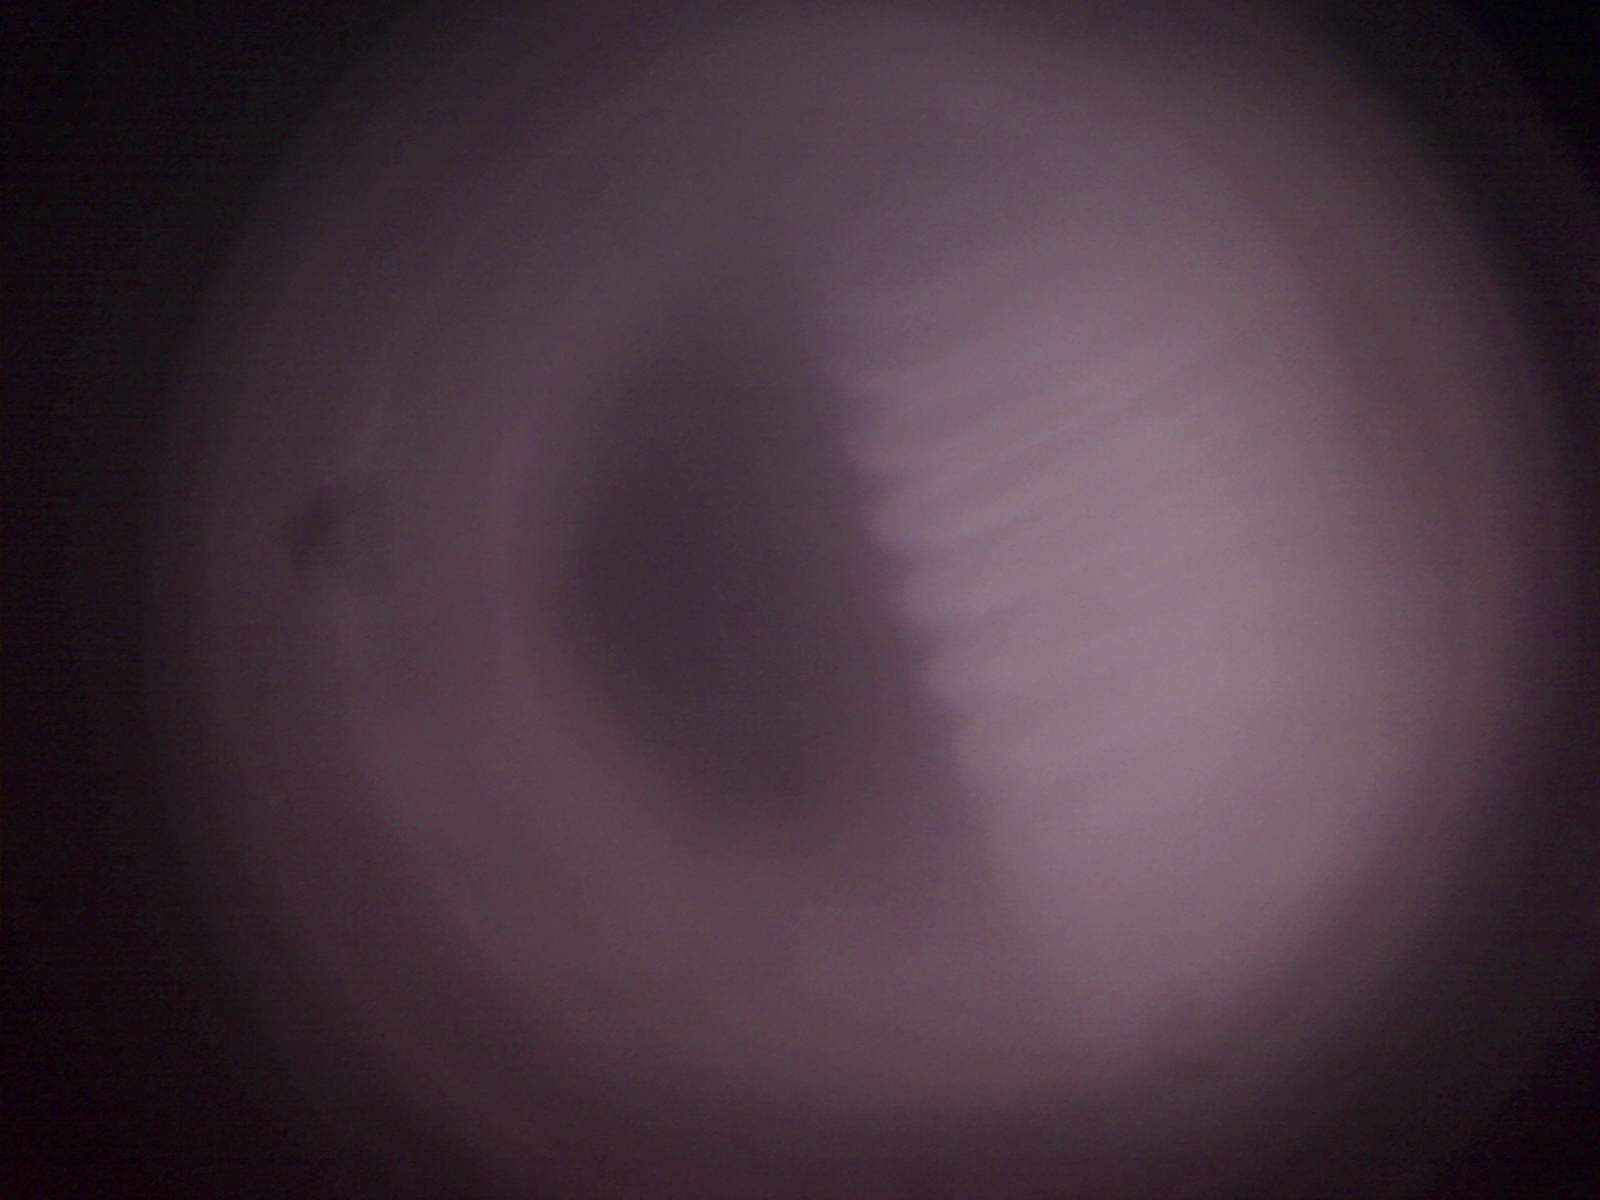
\includegraphics[width=\textwidth]{img/halogen_filament}
        \caption{Halogen source.}
    \end{subfigure}
    \begin{subfigure}[p]{0.30\textwidth}
        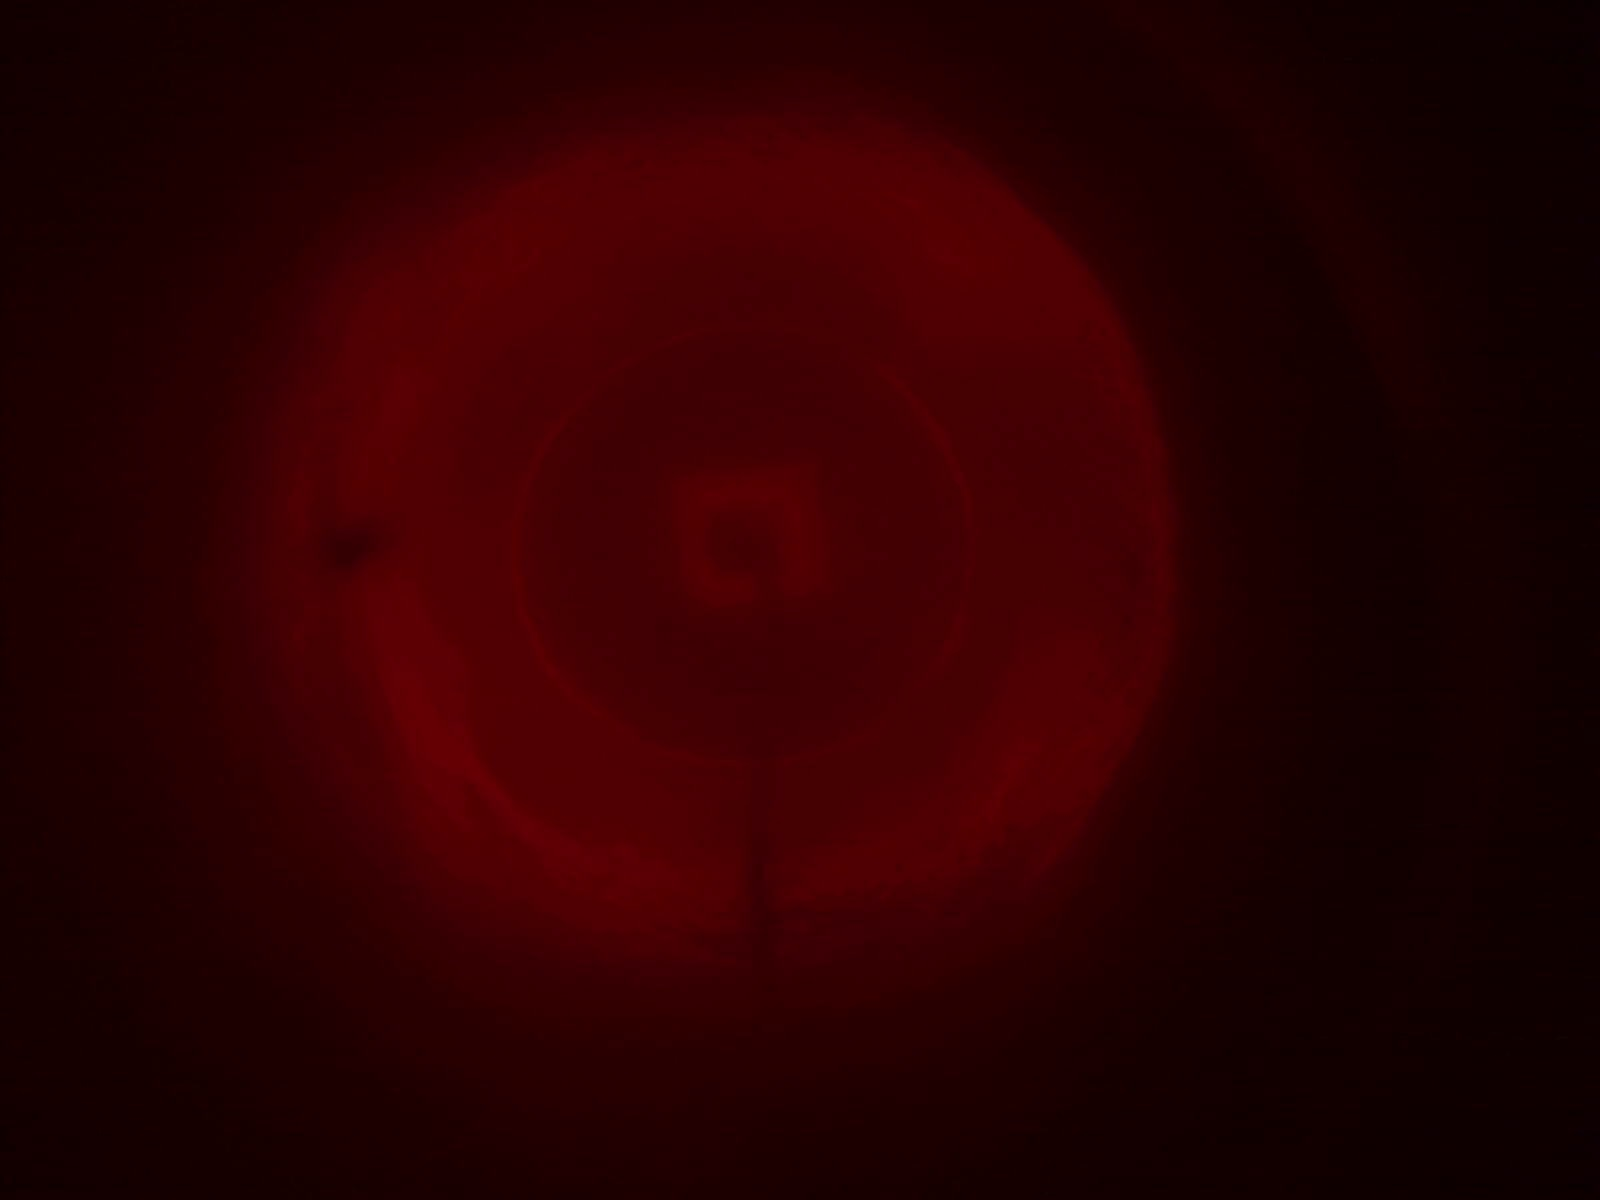
\includegraphics[width=\textwidth]{img/led_chip}
        \caption{LED source.}
    \end{subfigure}
    \begin{subfigure}[p]{0.30\textwidth}
        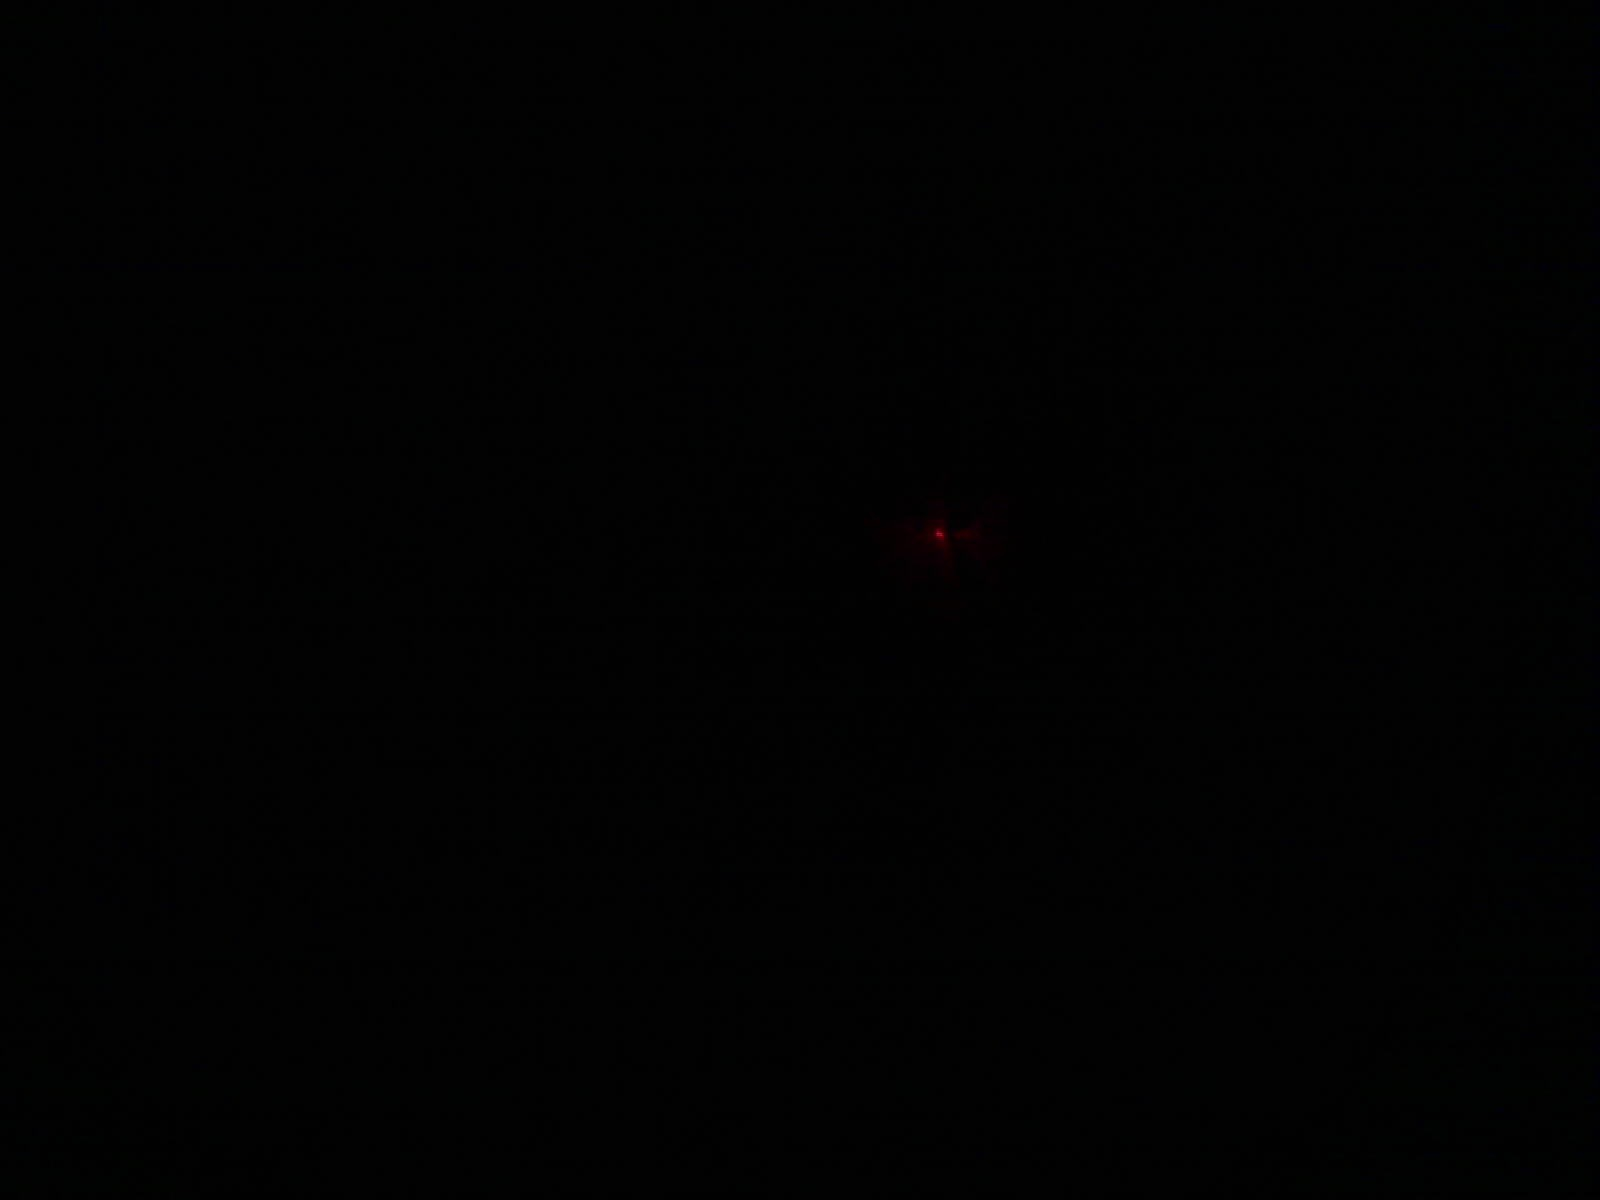
\includegraphics[width=\textwidth]{img/laser_aperture}
        \caption{Laser source.}
    \end{subfigure}
    \caption{Pictures taken in a 4f configuration.
        This means that both the object and the image are at a distance of 2f from the lens.
    So the magnification should be equal to 1.}
\label{fig:sources_4f}
\end{figure}

Again, we measure the diameters of the sources in pixels on the image and calculate the sizes of the sources in the object space.
We estimate a measurement error of $\Delta d_I = 20 \mbox{px} \hat{=} \SI{17}{\micro\meter}$ and $\Delta d_I = 2 \mbox{px} \hat{=} \SI{6}{\micro\meter}$ for the laser.

\begin{equation}
    d_O = d_I = d
    \label{equ:m_of_one}
\end{equation}

\begin{table}[h]
    \centering
    \begin{tabular}{l S[table-format=4.0] S[table-format=1.2] S[table-format=1.2] S[table-format=2.1]}
        \toprule
        source & {image space $d_I$ (px)} & {object space $d_O$ (\SI{}{\milli\meter})} & {$\Delta d_O$} & {error (\SI{}{\percent})} \\
        \midrule
        Halogen & 1150 & 3.26 & 0.02 &  6.1 \\
        LED     &  992 & 2.81 & 0.02 &  7.1 \\
        Laser   &   16 & 0.04 & 0.01 & 25   \\
        \bottomrule
    \end{tabular}
    \caption{Diameter of the source point measured in with the 4f configuration.}
\label{tab:diams_4f}
\end{table}

All the values obtained are smaller than the ones in the datasheet (\SI{4.8}{\milli\meter} for the halogen source, \SI{5}{\milli\meter} for the LED, and \SI{1.8}{\milli\meter} for the laser).
This is because it's really hard to determine the diameters with reflects on the lens and the reduction of exposure.
We note that values measured with the 4f system are smaller than with the first method.

\begin{figure}[H]
    \centering
    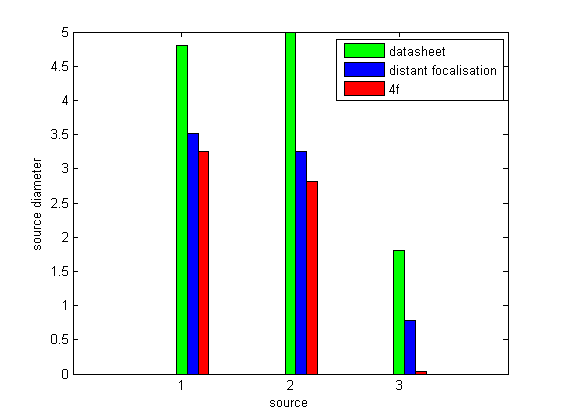
\includegraphics[width=0.7\textwidth]{img/source_diameters_graph}
    \caption{Source diameters.}
\label{fig:source_diameter_graph}
\end{figure}

\subsection{Light collection under different conditions}

We took pictures of the LED-source with the image being at different positions around the focal point and took to sum of the pixel's intensities to approximate the total energy of the image~(figure~\ref{fig:pixel_count}).
According to the \emph{brightness theorem}, the overall brightness should stay the same.
There could be several reasons to why this isn't exactly the case:
\begin{itemize}
    \item Non-linearity of the sensor and the camera's processing software
    \item Quantification errors
    \item The image overlaps the sensor when it's further away
    \item The LED isn't a perfect \emph{Lambertian emitter}
\end{itemize}

\begin{figure}[H]
    \centering
    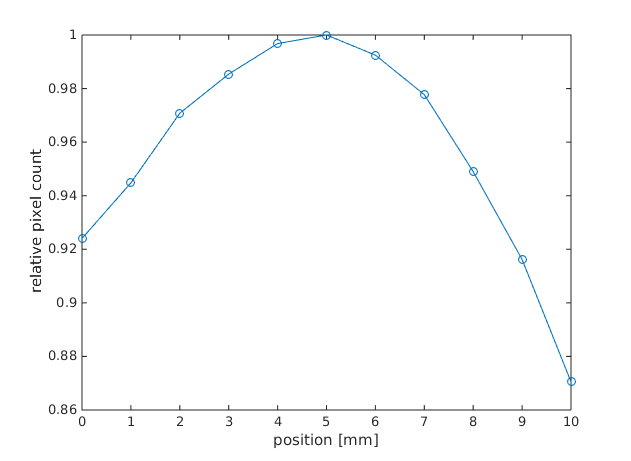
\includegraphics[width=0.9\textwidth]{img/pixel_count_position}
    \caption{Approximation of the total energy of the image with the sensor at different positions. It was in focus at \SI{5}{\milli\meter} and the energy clearly peaks at that point.}
\label{fig:pixel_count}
\end{figure}

\subsection{Spectral matching}

\begin{figure}[H]
    \centering
    \begin{subfigure}[p]{0.40\textwidth}
        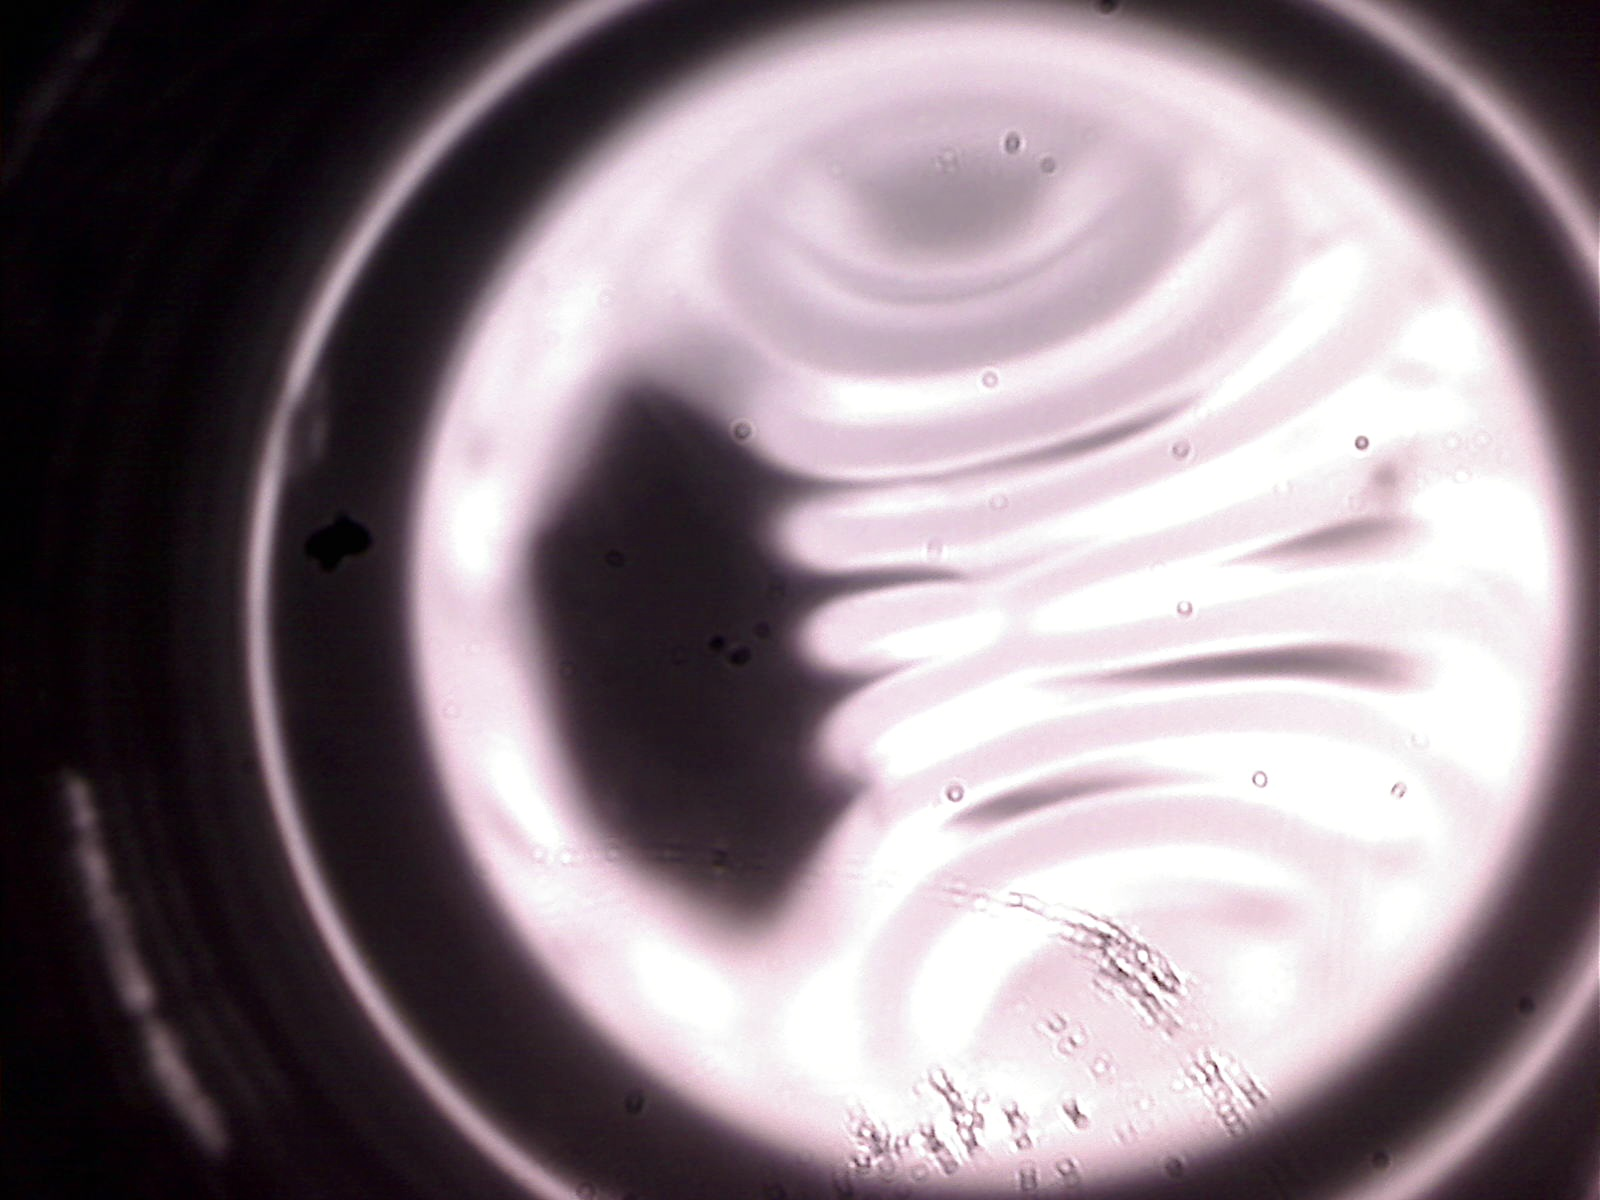
\includegraphics[width=\textwidth]{img/halogen_without_IR_filter.jpg}
        \caption{Image \emph{without} IR filter.}
    \end{subfigure}
    \begin{subfigure}[p]{0.40\textwidth}
        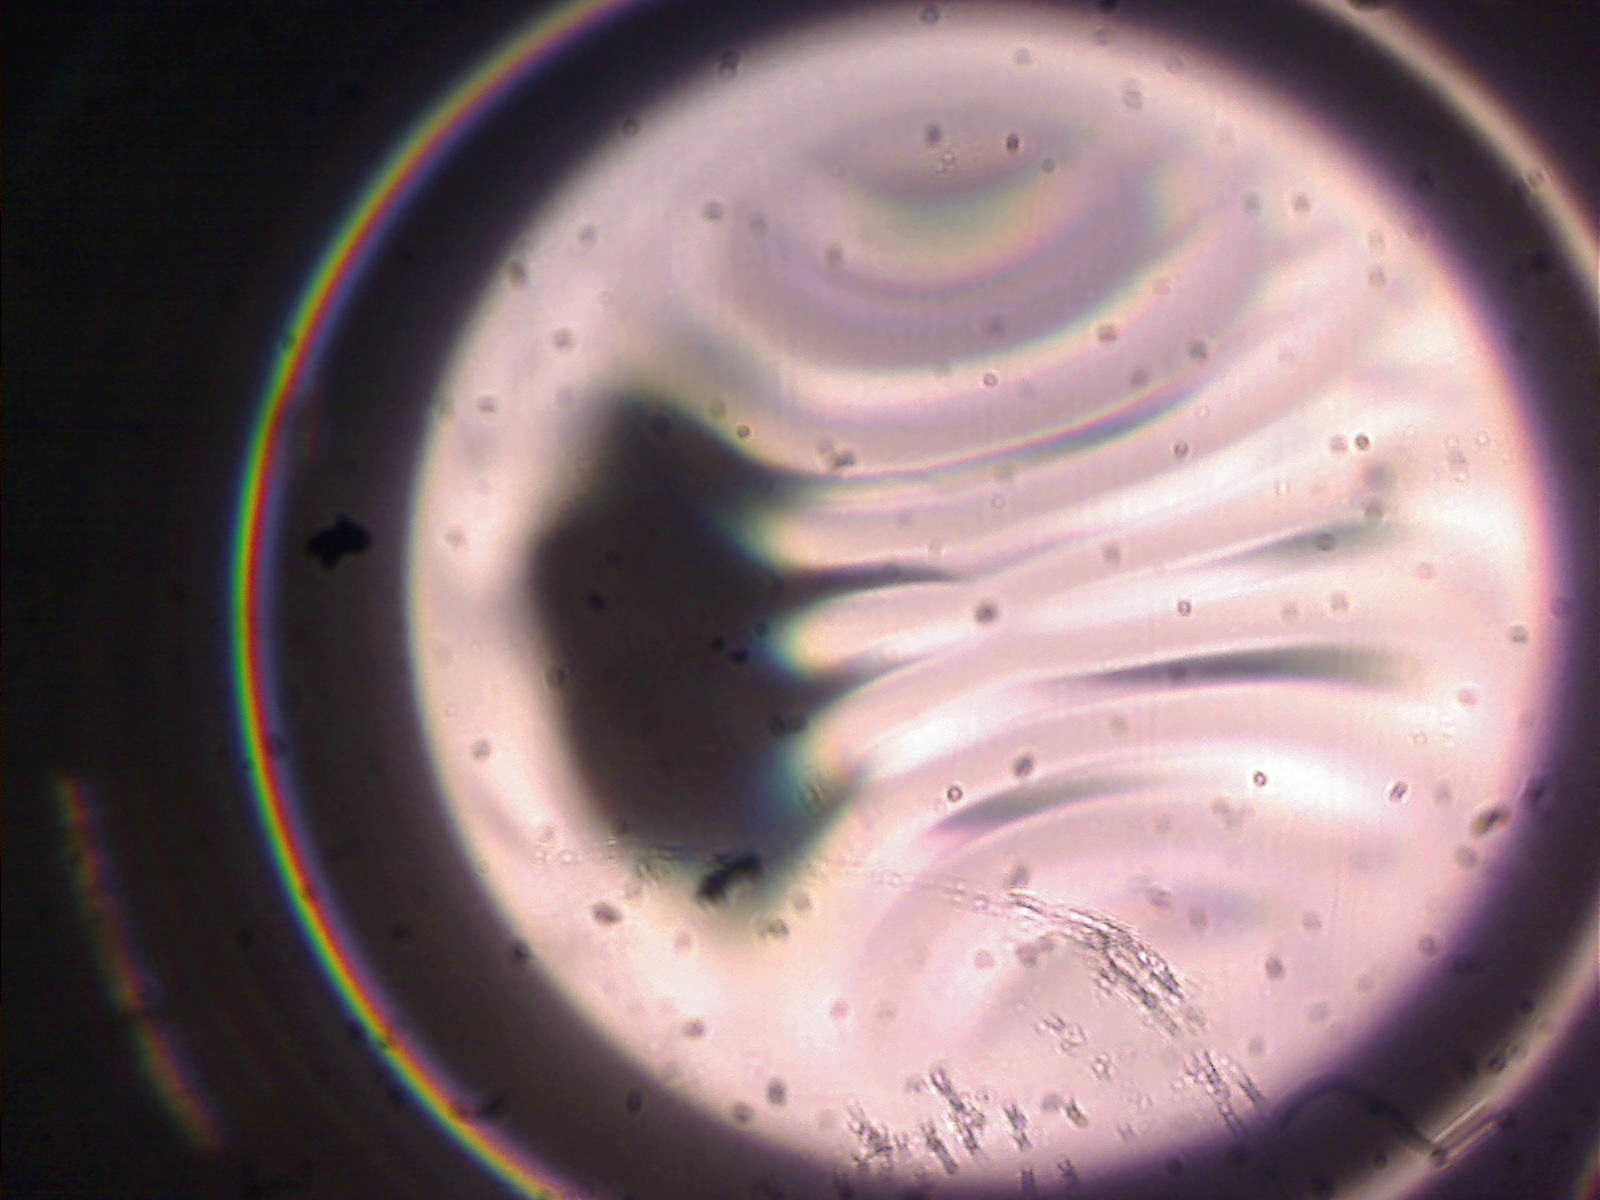
\includegraphics[width=\textwidth]{img/halogen_with_IR_filter.jpg}
        \caption{Image \emph{with} IR filter.}
    \end{subfigure}
    \begin{subfigure}[p]{0.40\textwidth}
        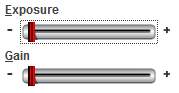
\includegraphics[width=\textwidth]{img/no_IR_filter}
        \caption{Exposure settings \emph{without} IR filter.}
    \end{subfigure}
    \begin{subfigure}[p]{0.40\textwidth}
        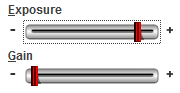
\includegraphics[width=\textwidth]{img/IR_filter}
        \caption{Exposure settings \emph{with} IR filter.}
    \end{subfigure}
    \caption{Image of the halogen lamp's filament with and without the IR filter in front of the sensor, and the according exposure settings. The fact that a longer exposure time is needed for about the same brightness with the IR filter in place shows that the lamp emits a lot of infrared light.}
\label{fig:saturation}
\end{figure}

\begin{figure}[H]
    \centering
    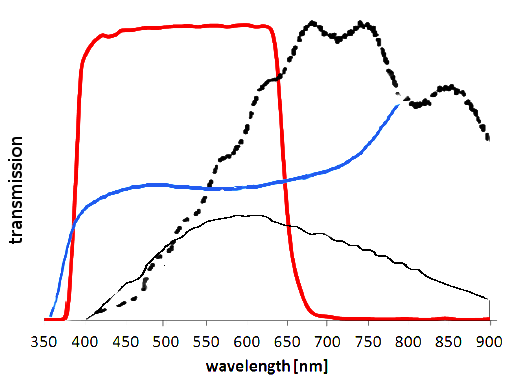
\includegraphics[width=0.40\textwidth]{img/transmissions}
    \caption{Sketch of the spectra of all components.
    Dashed: halogen source spectrum, black: detector spectral sensitivity, blue: polarizer transmission, red: IR filter transmission.
    The graph shows, that the halogen lamp emits a lot of light in the infrared spectrum and that the detector is still sensitive to it.
    The experiment showed exactly the same: A lot less exposure time and gain is needed when the IR filter is gone.
    What the graph doesn't show is the functionality of the polarizer with light in the IR spectrum (it drops almost to zero; which could also be reproduced in the experiment).}
\label{fig:transmissions}
\end{figure}

\subsection{Web example: Phillips Brite FL 300 ww N}

That is an \emph{OLED panel} used to light interior spaces that require beautiful and high performance lighting.
The lighting source is a panel of $\SI{102.4}{\milli\meter} \times \SI{102.4}{\milli\meter}$.
His luminous flux is up to 300 lumen and his efficacy up to \SI{50}{\lumen\per\watt}.
In normal conditions, the luminous flux decreases to approximately \SI{70}{\percent} after \SI{10000}{} hours, the voltage increases, and colors and homogeneity also change.

\begin{figure}[H]
    \centering
    \begin{subfigure}[p]{0.45\textwidth}
        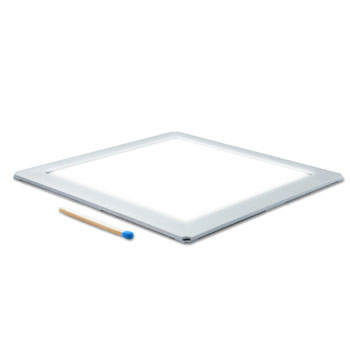
\includegraphics[width=\textwidth]{img/oled}
    \end{subfigure}
    \begin{subfigure}[p]{0.45\textwidth}
        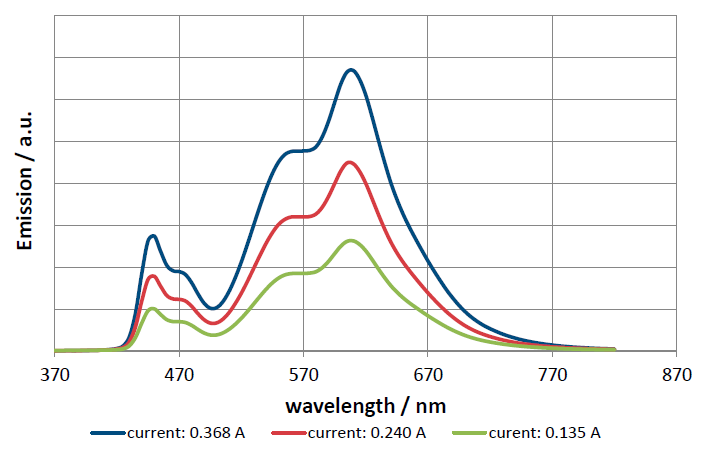
\includegraphics[width=\textwidth]{img/oled_emission}
    \end{subfigure}
    \caption{OLED panel and its emission spectrum.}
\label{fig:oled}
\end{figure}

\section{Discussion and conclusions}
We measured the sizes of several sources and discovered the problems associated with this kind of measurement; especially with the 4f configuration.
We also saw the importance of transmission matching in optical system design to get any useful results.

\end{document}
